\documentclass[conference]{IEEEtran}
\IEEEoverridecommandlockouts
\usepackage{cite}
\usepackage{amsmath,amssymb,amsfonts}
\usepackage{algorithmic}
\usepackage{graphicx}
\usepackage{textcomp}
\usepackage{xcolor}
\usepackage[utf8]{inputenc}
\usepackage{booktabs}
\usepackage{float}
\usepackage[portuguese]{babel}

\makeatletter
\newcommand{\linebreakand}{%
\end{@IEEEauthorhalign}
\hfill\mbox{}\par
\mbox{}\hfill\begin{@IEEEauthorhalign}
}
\makeatother

\def\BibTeX{{\rm B\kern-.05em{\sc i\kern-.025em b}\kern-.08em
		T\kern-.1667em\lower.7ex\hbox{E}\kern-.125emX}}

\begin{document}

\title{ANADI - Trabalho Prático 2:\\
Análise de Desempenho De Técnicas de Aprendizagem Automática}

\author{\IEEEauthorblockN{Fábio Borges\IEEEauthorrefmark{1}, Joel Ferreira\IEEEauthorrefmark{2}, Jorge Cruz\IEEEauthorrefmark{3}}
\IEEEauthorblockA{\textit{Departamento de Engenharia Informática}} \\
\textit{Instituto Superior de Engenharia do Porto}\\
\IEEEauthorrefmark{1} 1100719@isep.ipp.pt
\IEEEauthorrefmark{2} 1191843@isep.ipp.pt
\IEEEauthorrefmark{3} 1221715@isep.ipp.pt
}


\maketitle

\begin{abstract}
Este artigo tem como objetivo a aplicação de algoritmos de aprendizagem automática na exploração de dados e respetiva comparação usando os testes estatísticos mais adequados. A temática incide sobre os níveis de poluição e seus impactos em diversos países europeus, no âmbito da disciplina de Análise de Dados em Informática. 

Foram aplicados modelos de regressão e classificação para prever mortes prematuras e distinguir doenças respiratórias. Os modelos foram avaliados com métricas estatísticas e comparados entre si.
\end{abstract}

\begin{IEEEkeywords}
poluição, saúde, regressão linear, classificação, árvores de decisão, K-vizinhos-mais-próximos, redes neuronais, SVM.
\end{IEEEkeywords}

\section{Introdução}

Este artigo começa por fazer uma introdução aos conceitos teóricos relevantes para a execução do trabalho e que foram abordados na disciplina de ANADI, \textbf{nomeadamente distribuição de dados, testes, correlações, regressões e previsões. }

De seguida, na ótica dos dados do problema - a poluição, são descritos os métodos e resultados obtidos em cada problema proposto. 

Por último, são apresentadas as conclusões do  trabalho.

Foi utilizado o \textit{python} para tratamento e processamento dos dados.

\section{Introdução Teórica}

Nesta secção serão introduzidos os conceitos teóricos sobre os diferentes algoritmos e modelos desenvolvidos na resolução deste trabalho. 

\subsection{Regressão}

\subsubsection{Regressão linear}

%\paragraph{}

A regressão linear é uma técnica estatística usada para modelar a relação entre uma variável dependente e uma ou mais variáveis independentes. Quando há apenas uma variável explicativa, o modelo é denominado \textbf{regressão linear simples}, sendo representado pela equação:

\begin{equation}
	Y = \beta_0 + \beta_1 X + \varepsilon
\end{equation}

onde \( Y \) é a variável que tentamos prever, denominada variável dependente. \( X \) é a variável independente (ou preditora), \( \beta_0 \) e \( \beta_1 \) são os coeficientes do modelo, e \( \varepsilon \) representa o erro aleatório. \cite{madureira2024aed}

\subsubsection{Regressão linear múltipla}
A regressão linear múltipla é uma extensão da regressão linear simples, na qual há mais de uma variável independente. A equação do modelo assume a forma:

\begin{equation}
	Y = \beta_0 + \beta_1 X_1 + \beta_2 X_2 + \dots + \beta_n X_n + \varepsilon
\end{equation}

Para se poder aplicar a regressão linear múltipla é necessário que exista uma relação linear entre a variável objetivo (Y) e as variáveis preditoras, os resíduos da regressão devem seguir uma distribuição normal e não deve existir multicolineariadade.\cite{madureira2024aed}

\subsection{Métricas de avaliação de modelos de regressão}

As métricas MAE, MSE, RMSE e R$^2$ são utilizadas principalmente para avaliar as taxas de erro de previsão e o desempenho do modelo na análise de regressão.

\medskip
\subsubsection{Mean Absolute Error - MAE}
Erro absoluto médio, é a soma das diferenças absolutas entre as previsões e os valores reais, dividindo pelo número total de pontos de dados.


\begin{equation}
	MAE = \frac{1}{n} {\sum_{i=1}^{n} |y_i - \hat{y_i}|}
	 \label{MAEeq}
\end{equation}

\medskip
\subsubsection{Mean Squared Error - MSE}
Erro quadrático médio, representa a diferença entre os valores originais e os valores previstos extraídos através do quadrado da diferença média do conjunto de dados.

\medskip
\subsubsection{Root Mean Squared Error - RMSE}
Mede a magnitude média do erro, tomando a raiz quadrada da média das diferenças quadráticas entre a previsão ($\hat{y_i}$) e a observação efetiva ($y_i$).


\begin{equation}
	RMSE = \sqrt{\frac{1}{n} {\sum_{i=1}^{n} (y_i - \hat{y_i})^2}}
	\label{RMSEeq}
\end{equation}

O RMSE é uma boa medida de exatidão, mas apenas para comparar erros de previsão de diferentes modelos ou configurações de modelos para uma determinada variável e não entre variáveis, uma vez que é dependente da escala. 

\medskip
\subsubsection{R$^2$ - Coeficiente de Determinação}

Representa o coeficiente de determinação dos valores em comparação com os valores originais. O valor de 0 a 1 é interpretado como percentagem. Quanto mais elevado for o valor, melhor é o modelo.\cite{madureira2024cv} 


\subsection{Árvores de Decisão}

Uma árvore de decisão,  \figurename~\ref{fig:Decision_Trees_example},  consiste num conjunto de nós de decisão, ligados por ramos, que se estendem para baixo a partir do nó raiz até terminarem em nós folha. 

Começando no nó raiz, que por convenção é colocado no topo do diagrama de árvore de decisão, as variáveis são testadas nos nós de decisão, sendo que cada resultado possível resulta num ramo. Cada ramo conduz então a outro nó de decisão ou a um nó folha terminal. 

A aprendizagem em árvore de decisão é um método de aproximação de uma função-alvo de valor discreto representada numa árvore de decisão. \cite{madureira2024dt}

\begin{figure}[h]
	\centering
	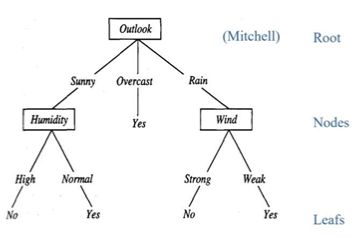
\includegraphics[width=0.5\linewidth]{Decision_Trees_example}
	\caption{Exemplo de árvore de decisão. \cite{madureira2024dt}}
	\label{fig:Decision_Trees_example}
\end{figure}

\subsubsection{Árvore de Decisão - Regressão}

As árvores de regressão são utilizados para prever variáveis-alvo contínuas, como o preço de uma casa ou o número de clientes que visitarão uma loja num determinado dia. Para fazer uma previsão, o regressor da árvore de decisão percorre a árvore desde o nó raiz até ao nó folha que corresponde às caraterísticas do novo ponto de dados. O valor previsto é então o valor médio da variável alvo para todos os pontos de dados no nó folha. \cite{ohekar_what_2023}

\medskip
\subsubsection{Árvore de Decisão - Classificação}

Os classificadores de árvores de decisão são utilizados para prever variáveis-alvo categóricas, como, por exemplo, se uma mensagem de correio eletrónico é ou não spam ou se um cliente vai ou não desistir. Para efetuar uma previsão, o classificador de árvore de decisão percorre a árvore desde o nó raiz até ao nó folha que corresponde às caraterísticas do novo ponto de dados. A classe prevista é então a classe com a maioria dos pontos de dados no nó folha. \cite{ohekar_what_2023}

\subsection{Cross-Validation}

A validação cruzada (Cross-Validation) é um método estatístico de avaliação e comparação de algoritmos de aprendizagem, dividindo os dados em dois segmentos: um utilizado para treinar um modelo e o outro utilizado para validar o modelo. Na validação cruzada típica, os conjuntos de treino e validação devem cruzar-se em rondas sucessivas, de modo a que cada ponto de dados tenha uma hipótese de ser validado. \cite{refaeilzadeh_cross-validation_2009}

\medskip
\subsubsection{Hold Out}

Esta abordagem consiste em dividir aleatoriamente os dados em dois conjuntos: um conjunto é utilizado para treinar o modelo e o outro conjunto é utilizado para testar o modelo. O processo funciona da seguinte forma: 
\begin{itemize}
	\item Construir (treinar) o modelo no conjunto de dados de treino; 
	\item Aplicar o modelo ao conjunto de dados de teste para prever o resultado de novas observações não vistas; 
	\item Quantificar o erro de previsão como a diferença média quadrática entre os valores de resultados observados e previstos. \cite{madureira2024cv}
\end{itemize}

\medskip
\subsubsection{K-Fold Cross-Validation}

O método de validação cruzada \textit{k-fold} avalia o desempenho do modelo em diferentes subconjuntos dos dados de treino e, em seguida, calcula a taxa média de erro de previsão. O algoritmo é o seguinte:
\begin{enumerate}
	\item Dividir aleatoriamente o conjunto de dados em \textit{k} subconjuntos (ou \textit{k-fold}) (por exemplo, 5 subconjuntos);
	\item Reservar um subconjunto e treinar o modelo em todos os outros subconjuntos;
	\item Testar o modelo no subconjunto reservado e registar o erro de previsão;
	\item Repetir este processo até que cada um dos \textit{k} subconjuntos tenha servido como conjunto de teste; 
	\item Calcular a média dos \textit{k} erros registados. Este é o chamado erro de validação cruzada, que serve de métrica de desempenho para o modelo. 
\end{enumerate}

A validação cruzada \textit{K-fold} (CV) é um método robusto para estimar a exatidão de um modelo. \cite{madureira2024cv}

\subsection{Redes Neuronais}

Uma rede neuronal, \figurename~\ref{fig:nn}, consiste numa rede de neurónios artificiais ou nós, em camadas, com alimentação direta e completamente ligada:

\begin{itemize}
	\item A natureza \textit{feedforward} da rede restringe-a uma única direção de fluxo e não permite ciclos. 
	\item A maioria das redes é constituída por três camadas: uma camada de entrada, uma camada oculta e uma camada de saída; 
	\begin{itemize}
		\item Pode haver mais de uma camada oculta, embora a maioria das redes contenha apenas uma, o que é suficiente para a maioria das finalidades.
	\end{itemize}
	
	  
	\item  A rede neuronal está completamente ligada, o que significa que cada nó de uma determinada camada está ligado a todos os nós das camadas adjacentes, mas não a outros nós da mesma camada:
	\begin{itemize}
		\item Cada conexão entre nós tem um peso (por exemplo, $w_{11}$) associado.
		\item  Na inicialização, estes pesos são atribuídos aleatoriamente a valores entre 0 e 1. \cite{madureira2024nn}
	\end{itemize}
\end{itemize}

\begin{figure}
	\centering
	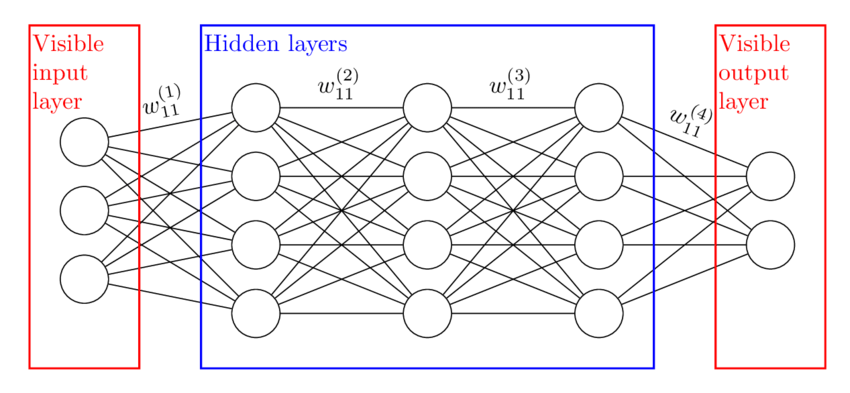
\includegraphics[width=0.7\linewidth]{NN}
	\caption{Exemplo de rede neuronal.}
	\label{fig:nn}
\end{figure}



\subsection{Support Vector Machines - SVM}

Uma máquina de vetores de suporte (SVM) é um algoritmo de aprendizagem automática supervisionada utilizado tanto para a classificação como para a regressão. Embora também se fale de problemas de regressão, é mais adequado para a classificação. O principal objetivo do algoritmo SVM é encontrar o hiperplano ideal num espaço N-dimensional que possa separar os pontos de dados em diferentes classes no espaço de caraterísticas, \figurename~\ref{fig:svm}. O hiperplano tenta que a margem entre os pontos mais próximos das diferentes classes seja a máxima possível. A dimensão do hiperplano depende do número de caraterísticas. Se o número de caraterísticas de entrada for dois, então o hiperplano é apenas uma linha. Se o número de caraterísticas de entrada for três, então o hiperplano torna-se num plano 2-D. \cite{madureira2024svm}

Terminologia:

\begin{itemize}
	\item \textbf{Hiperplano}: Um limite de decisão que separa diferentes classes no espaço de caraterísticas e é representado pela equação $wx + b = 0$ na classificação linear.
	
	\item \textbf{Vetores de suporte}: Os pontos de dados mais próximos do hiperplano, cruciais para determinar o hiperplano e a margem no SVM.
	
	\item \textbf{Margem}: A distância entre o hiperplano e os vetores de suporte. O objetivo do SVM é maximizar esta margem para obter um melhor desempenho de classificação.
	
	\item \textbf{Kernel}: Uma função que mapeia os dados para um espaço de dimensão superior, permitindo que o SVM lide com dados não linearmente separáveis. \cite{madureira2024svm}
\end{itemize}

\begin{figure}
	\centering
	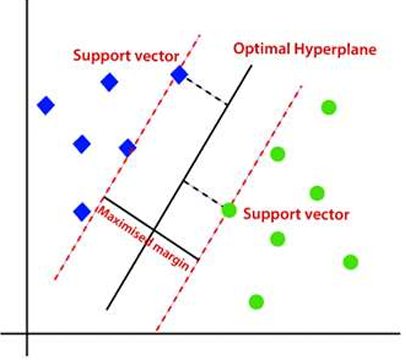
\includegraphics[width=0.5\linewidth]{svm}
	\caption{Hiperplano, vetores de suporte e margem - SVM.}
	\label{fig:svm}
\end{figure}


\subsection{kNN - K-Vizinhos Mais Próximos}


O algoritmo do vizinho mais próximo (\textit{Nearest Neighbour}) classifica uma instância de dados com base nos seus vizinhos. A classe de uma instância de dados determinada pelo algoritmo dos k-vizinhos mais próximos é a classe com maior representação entre os k-vizinhos mais próximos. 

Os algoritmos do vizinho mais próximo estão entre os algoritmos de aprendizagem automática supervisionada mais “simples” e têm sido bem estudados no domínio do reconhecimento de padrões. 

O algoritmo do k-vizinho mais próximo é usado em projetos de classificação como referência de desempenho preditivo quando se está a tentar desenvolver modelos mais sofisticados. O kNN funciona utilizando a proximidade e a votação por maioria para efetuar previsões. \cite{madureira2024knn}

\section{Métodos e Resultados Obtidos}

\subsection{Análise Exploratória de Dados}
\medskip
\subsubsection{\textbf{Exercício 4.1.1}}

Neste exercício era pretendido o carregamento dos dados, a sua dimensão e respetivo sumário. 
Começamos então por carregar os dados provenientes do ficheiro AIRPOL\_data. Verificamos que o mesmo possui 49140 linhas e 16 colunas. De seguida, através da função df.info(), foi possível verificar a existência de colunas vazias ("Unnamed"), que foram eliminadas. Com a função df.describe(), obtivemos a análise estatística representada na figura \ref{fig:Statistics}.

\begin{figure}[H]
	\centering
	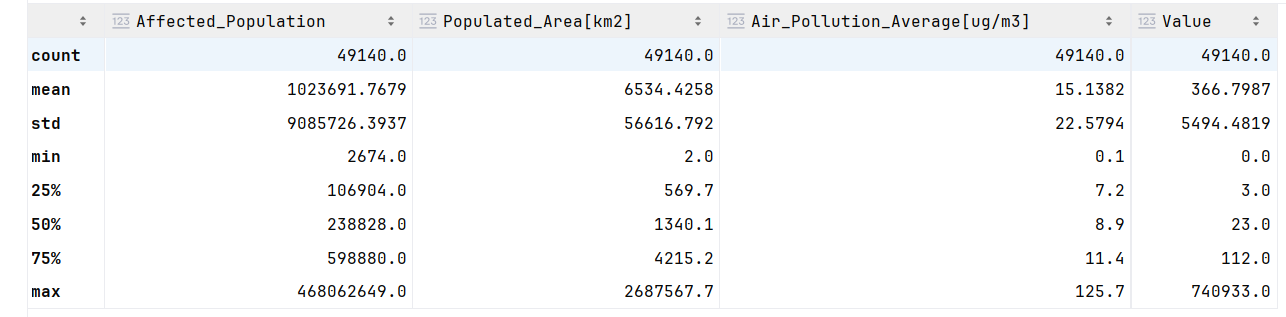
\includegraphics[width=1\linewidth]{statistics}
	\caption{Resumo estatístico do Dataframe}
	\label{fig:Statistics}
\end{figure}


\medskip
\subsubsection{\textbf{Exercício 4.1.2}}

Pretendia-se a exploração dos dados com os gráficos mais adequados. Em primeiro lugar identificamos as variáveis previsoras e as varáveis alvo. Relativamente às variáveis previsoras temos: 'Affected\_Population', 'Populated\_Area[km2]', 'Air\_Pollution\_Average[ug/m3]', 'Country', 'NUTS\_Code' e 'Air\_Pollutant'. Destas, 'Affected\_Population', 'Populated\_Area[km2]', 'Air\_Pollution\_Average[ug/m3]' eram variáveis contínuas pelo que recorremos à utilização de histogramas e \textit{boxplots} para visualizar as suas distribuições. Concluímos que todas elas apresentam distribuições próximas da distribuição normal com a presença considerável de \textit{outliers}. Esses \textit{outliers} levaram a uma necessidade de analisar mais detalhadamente estes dados por país e por poluente pois estas variações podem estar relacionadas com esses fatores. 

\begin{figure}[H]
	\centering
	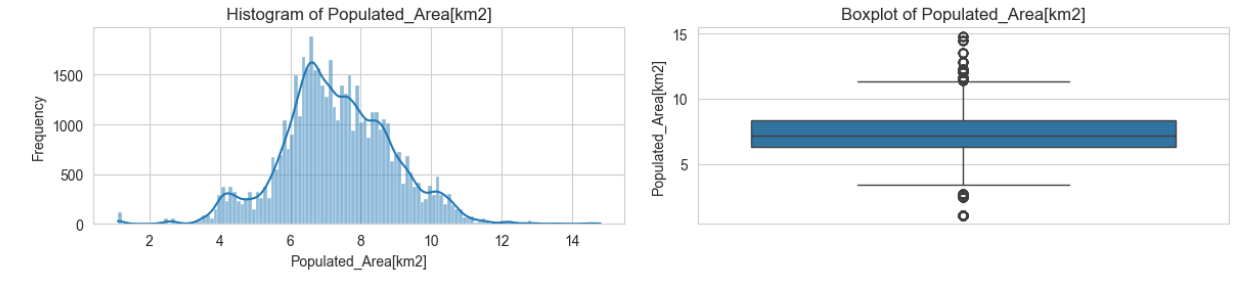
\includegraphics[width=1\linewidth]{PopArea}
	\caption{Distribuição da variável 'Populated Area[km2]'}
	\label{fig:PopArea}
\end{figure}

De seguida, analisamos as variáveis previsoras discretas ('Country', 'NUTS\_Code' e 'Air\_Pollutant') e verificamos que os países com mais dados disponíveis são Alemanha, Itália e França por esta ordem. Denotamos também a existência de um número consideravelmente superior de registos para o poluente PM2.5, seguindo-se o poluente NO2 e O3.

Relativamente à relação das variáveis 'Affected\_Population', 'Populated\_Area[km2]', 'Air\_Pollution\_Average[ug/m3]' com o país, 'NUTS\_Code' e poluente, tiramos as seguintes conclusões:
\begin{itemize}
	\item Para as variáveis população afetada, área populacional e poluição média do ar, verificam-se diferenças nas distribuições destes valores por país, o que poderá justificar a grande presença de outliers quando analisámos estas variáveis individualmente.
	\item Todas as variáveis apresentam um elevado número de outliers por país, com destaque para a variável poluição média do ar, onde a quantidade de outliers se destaca em relação às outras variáveis numéricas.
	\item Desta visualização, há que salientar os elevados valores de poluição média[ug/m3] para o poluente O3 em relação aos outros dois poluentes.  
\end{itemize}

\begin{figure}[h]
	\centering
	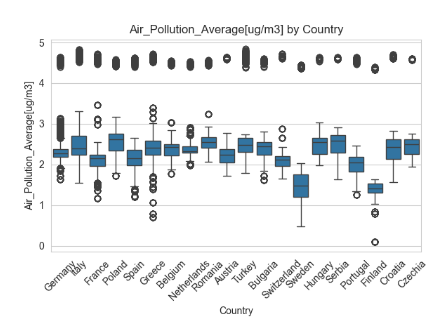
\includegraphics[width=0.8\linewidth]{AirPollutionAvgByCountry}
	\caption{Distribuição de 'Air Pollution Average' por país}
	\label{fig:AvgByCountry}
\end{figure}

\begin{figure}[H]
	\centering
	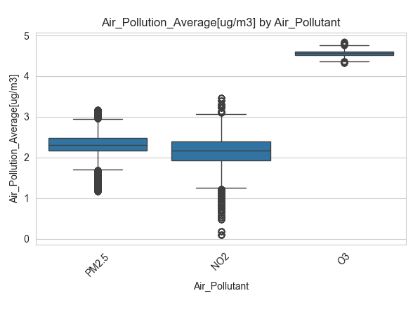
\includegraphics[width=0.8\linewidth]{AirPollutionAvgByPollutant}
	\caption{Distribuição de 'Air Pollution Average' por poluente}
	\label{fig:AvgByPollutant}
\end{figure}

Da análise das varáveis alvo (Doença associada ao poluente e Mortes prematuras), concluímos:
\begin{itemize}
	\item Relativamente às doenças registadas, ocorreram mais registos de Asma, AVC e Diabetes.
	\item A variável 'Value' correspondente às mortes prematuras apresenta uma distribuição assimétrica à direita, o que resulta numa elevada concentrção de valores baixos.
\end{itemize}

\begin{figure}[H]
	\centering
	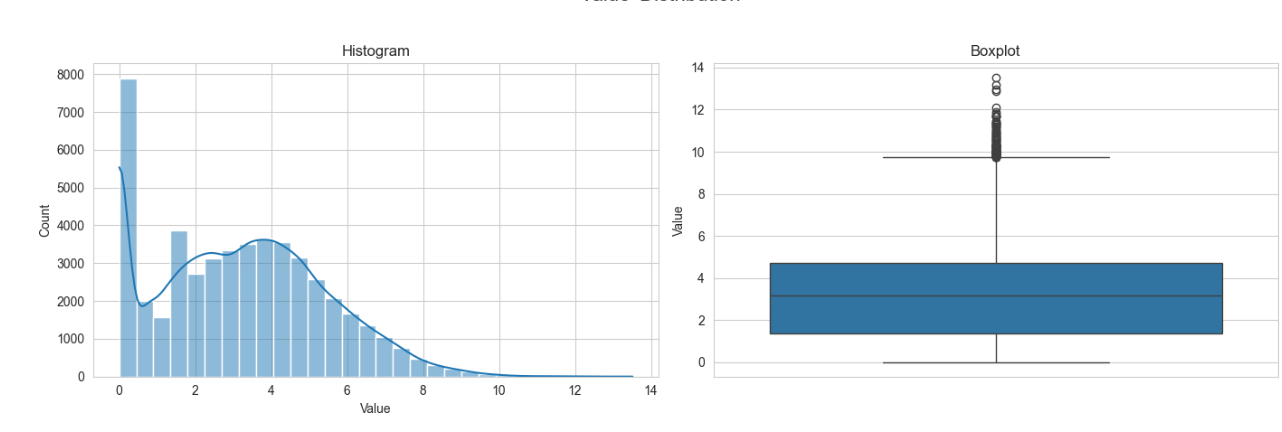
\includegraphics[width=0.8\linewidth]{ValueDist}
	\caption{Distribuição de 'Value' (Mortes prematuras)}
	\label{fig:AvgByCountry}
\end{figure}

Por último foi realizada uma análise bivariada onde cruzamos informação de variáveis previsoras com variáveis alvo. Desta análise obtivemos as seguintes conclusões:
\begin{itemize}
	\item Relativamente à relação entre as doenças e o nível médio de poluente no ar[ug/m3], verifica-se que este apresenta valores semelhantes em todas as doenças com exceção da doença pulmonar crónica onde os dados mostram que para esta doença, os níveis de poluente são mais elevados.
	\item Verificou-se também que o valores mais elevados do nível médio de poluente, não produzem necessariamente mais mortes prematuras. É possível verificar pelo gráfico que cruza as informações relativamente ao nível de poluente e ao número de mortes prematuras, que o poluente O3 apresenta os valores mais elevados em termos de concentração média do poluente mas é o que produz menos mortes. Já no caso do PM2.5, verificamos exatamente o contrário: valores menores e mais mortes prematuras.
\end{itemize}

\begin{figure}[H]
	\centering
	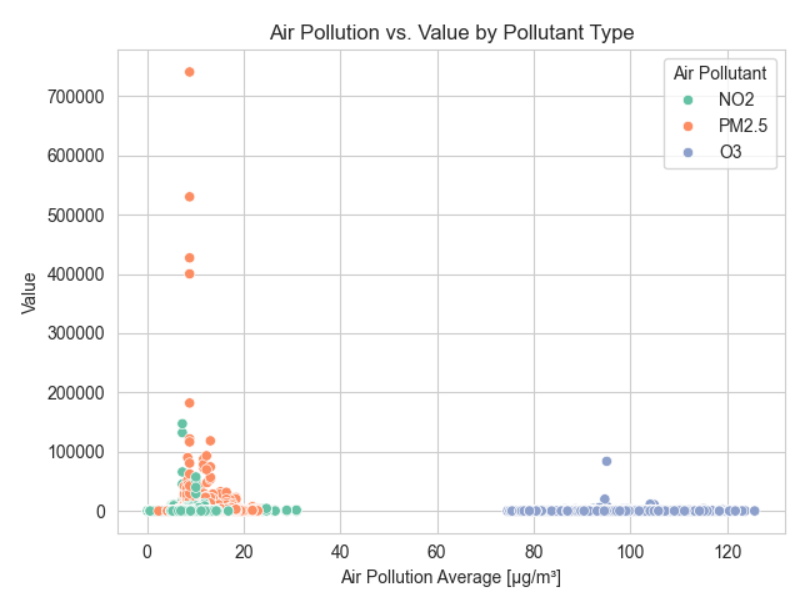
\includegraphics[width=0.8\linewidth]{AirPolValuePollutant}
	\caption{Poluente vs. Mortes prematuras}
	\label{fig:AvgByPollutant}
\end{figure}



\medskip
\subsubsection{\textbf{Exercício 4.1.3}}

Na fase de pré-processamento de dados foram seguidos os seguintes passos: eliminação de dados vazios, eliminação de dados duplicados e remoção de outliers. 

Da análise realizada anteriormente, verificamos uma grande presença de outliers nas variáveis 'Value' e 'Air Pollution Average[ug/m3]'.
Desta forma, decidimos eliminar os outliers destas duas variáveis para obtermos dados mais fiáveis e ao mesmo tempo não restringir o dataset de forma significativa. 

Para a variável 'Air Pollution Average[ug/m3]', inicialmente procedeu-se à eliminação dos outliers por país. No entanto, devido aos elevados valores desta variável para o poluente O3, os dados para este mesmo poluente eram completamente eliminados. A solução passou por eliminar os outliers por poluente e não por país. Isto resultou na permanência de um elevado número de outliers por país que serão referentes às concentrações para o poluente O3.

\medskip
\subsubsection{\textbf{Exercício 4.1.4}}

Neste exercício era pretendida a divisão dos países por regiões. Foi então utilizado um mapa de países por regiões, sendo criada uma nova coluna, 'Region' que guarda a respetiva região para o país considerado.

\medskip
\subsection{Regressão}

Esta seção apresenta uma análise detalhada da aplicação de modelos de regressão para prever mortes prematuras (\textit{Premature\_Deaths}) em países do sul da Europa (Grécia, Espanha, Itália e Portugal), utilizando o conjunto de dados \textit{AIRPOL\_data}. A análise inclui a exploração de correlações, a implementação de modelos de regressão (Regressão Linear Simples, Regressão Linear Múltipla, Árvore de Regressão, SVM e MLPRegressor), e a comparação estatística dos melhores modelos. Os resultados são apresentados com métricas de desempenho, funções de regressão, parâmetros otimizados e figuras ilustrativas.

\medskip
\subsubsection{\textbf{Exercício 4.2.1 - Análise de Correlação}}

A análise de correlação foi conduzida utilizando o coeficiente de Spearman para avaliar a relação entre \textit{Premature\_Deaths} e variáveis preditoras, incluindo \textit{Affected\_Population}, \textit{Populated\_Area[km2]}, \textit{Air\_Pollution\_Average[ug/m3]}, e variáveis categóricas codificadas (\textit{Air\_Pollutant} e \textit{Outcome}). O método de Spearman foi escolhido devido à presença de distribuições não normais, conforme identificado na análise exploratória.

% Resultados da correlação
A matriz de correlação, ilustrada na \figurename~\ref{fig:correlation_heatmap}, revela que \textit{Affected\_Population} apresenta a maior correlação positiva com \textit{Premature\_Deaths} (coeficiente próximo de 0,5), indicando que áreas com maior população afetada tendem a registrar mais mortes prematuras. A variável \textit{Air\_Pollution\_Average[ug/m3]} mostrou correlação moderada, enquanto \textit{Populated\_Area[km2]} apresentou correlação fraca. Entre os poluentes, o PM2.5 demonstrou maior associação com mortes prematuras, seguido por NO2, enquanto O3 apresentou correlação negativa. Doenças como Asma e AVC exibiram correlações positivas significativas, conforme destacado no gráfico de barras da \figurename~\ref{fig:correlation_bar}. Estas observações reforçam a influência da densidade populacional e de poluentes específicos na mortalidade prematura, justificando sua inclusão nos modelos de regressão.

\begin{figure}[h]
	\centering
	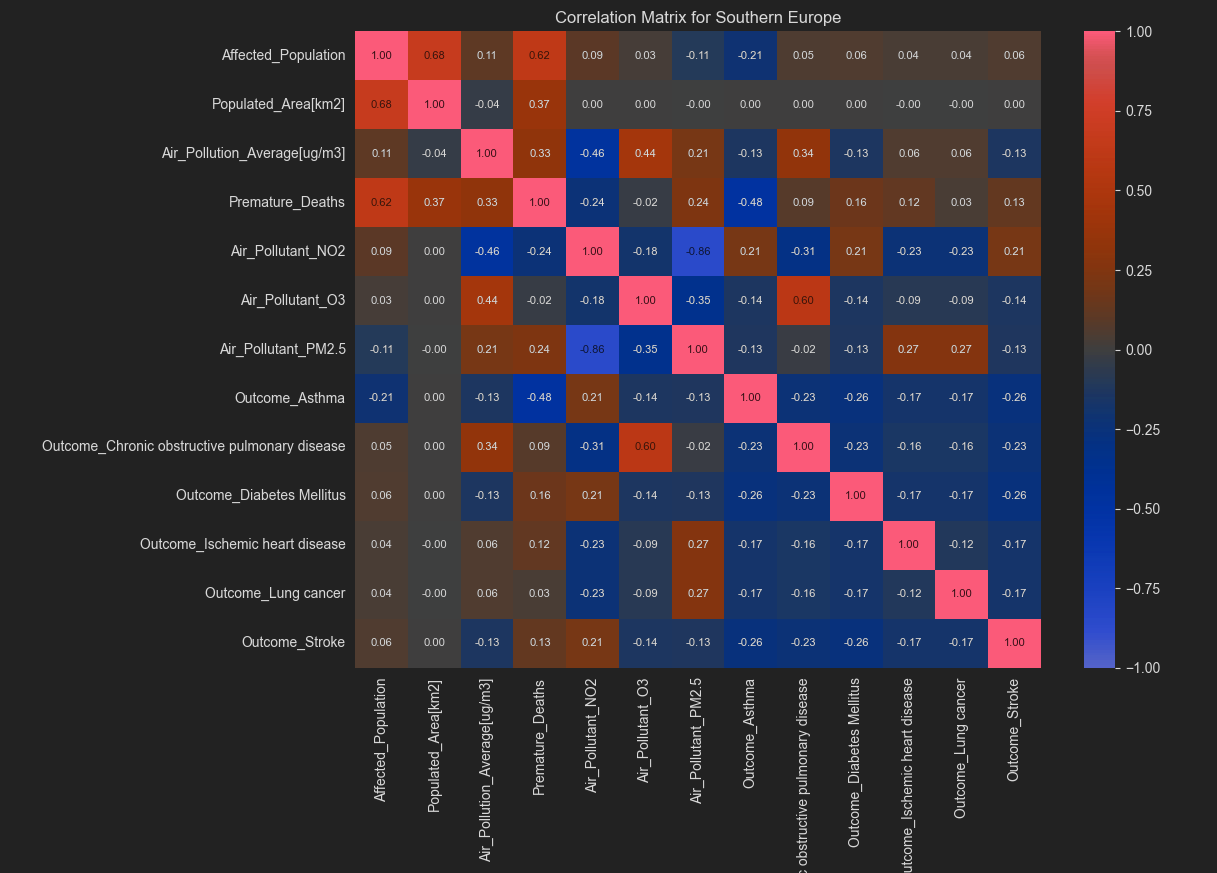
\includegraphics[width=0.9\linewidth]{matrix_correlacao}
	\caption{Matriz de correlação (Spearman) para variáveis preditoras e \textit{Premature\_Deaths} no sul da Europa.}
	\label{fig:correlation_heatmap}
\end{figure}

\begin{figure}[h]
	\centering
	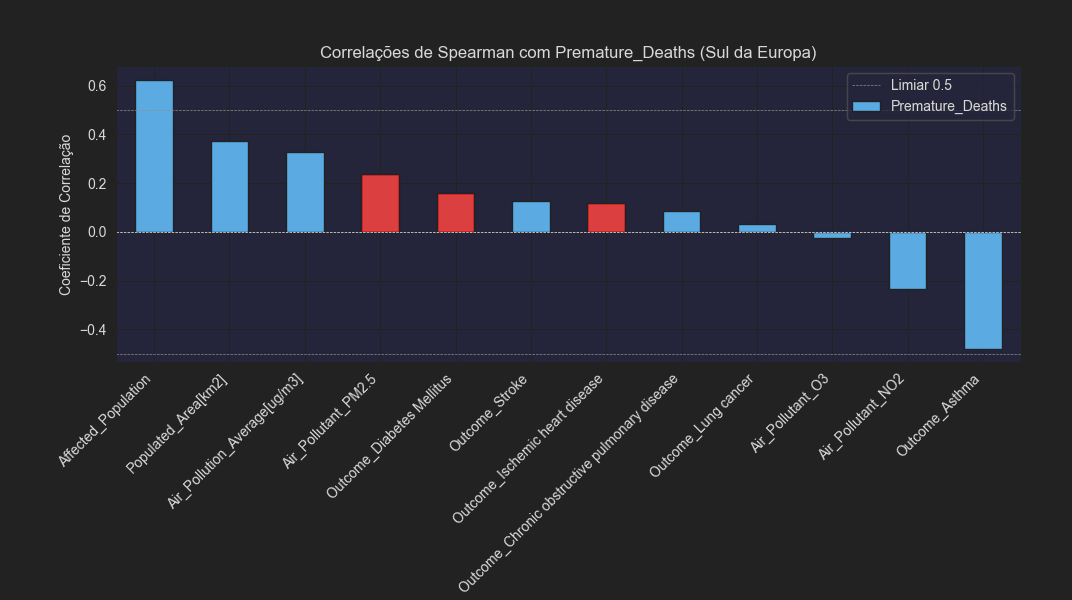
\includegraphics[width=0.9\linewidth]{correlacao_barras}
	\caption{Correlações de Spearman com \textit{Premature\_Deaths}, destacando \textit{Affected\_Population} e poluentes como PM2.5.}
	\label{fig:correlation_bar}
\end{figure}


% Visão geral dos modelos
Foram implementados os seguintes modelos: Regressão Linear Simples, Regressão Linear Múltipla, Árvore de Regressão, Support Vector Machine (SVM) e MLPRegressor (Rede Neural). Cada modelo foi avaliado utilizando validação cruzada \textit{k-fold} (k=5), com métricas de Erro Médio Absoluto (MAE), Raiz do Erro Quadrático Médio (RMSE) e Coeficiente de Determinação (R²). Os dados foram normalizados para garantir comparabilidade, especialmente para SVM e MLPRegressor, que são sensíveis à escala.

\medskip
\subsubsection{\textbf{Exercício 4.2.2 - Regressão Linear Simples}}

% Função e métricas
A Regressão Linear Simples foi aplicada considerando apenas \textit{Affected\_Population} como preditor. A função obtida é:

\begin{equation}
	\text{Premature\_Deaths} = 0{,}224 \cdot \text{Affected\_Population} - 0{,}000
\end{equation}

As métricas de desempenho, obtidas via validação cruzada, são: MAE médio de 0,005 (desvio padrão 0,000), RMSE médio de 0,022 (desvio padrão 0,004) e R² de 0,317. Estes resultados indicam que o modelo explica 31,7\% da variância, mas é limitado por considerar apenas uma variável preditora.

\medskip
\subsubsection{\textbf{Exercício 4.2.3a - Regressão Linear Multipla}}

% Função da regressão múltipla
A Regressão Linear Múltipla incorporou múltiplas variáveis preditoras, resultando na seguinte função:

Premature\_Deaths = -0.016 + (0.166) * Affected\_Population 

+ (0.065) * Populated\_Area[km2] 

+ (0.048) * Air\_Pollution\_Average[ug/m3] 

+ (0.010) * Air\_Pollutant\_NO2 

+ (-0.024) * Air\_Pollutant\_O3 

+ (0.014) * Air\_Pollutant\_PM2.5 

+ (-0.003) * Outcome\_Asthma 

+ (-0.002) * Outcome\_Chronic obstructive pulmonary disease 

+ (0.002) * Outcome\_Diabetes Mellitus 

+ (0.002) * Outcome\_Ischemic heart disease 

+ (0.000) * Outcome\_Lung cancer 

+ (0.001) * Outcome\_Stroke

\medskip

% Métricas e MAE fold-wise
Os MAE \textit{fold-wise} foram: [0,005541, 0,005972, 0,006128, 0,006050, 0,005922]. As métricas de desempenho são: MAE médio de 0,006 (desvio padrão 0,000), RMSE médio de 0,022 (desvio padrão 0,004) e R² de 0,338. O modelo explica 33,8\% da variância, superando a regressão simples, mas ainda limitado por relações não lineares.

\medskip
\subsubsection{\textbf{Exercício 4.2.3b - Árvore de Regressão}}

% Parâmetros e métricas
A Árvore de Regressão foi otimizada com os parâmetros: \texttt{max\_depth=7} e \texttt{min\_samples\_split=10}. Os MAE \textit{fold-wise} foram: [0,004656, 0,004834, 0,004450, 0,004857, 0,004878]. As métricas de desempenho são: MAE médio de 0,005 (desvio padrão 0,000), RMSE médio de 0,024 (desvio padrão 0,004) e R² de aproximadamente 0,350. O MAE inferior indica alta precisão média, mas o RMSE maior sugere sensibilidade a outliers.

\medskip
\subsubsection{\textbf{Exercício 4.2.3c - SVM}}

% Parâmetros e métricas
O SVM, com kernel RBF, foi otimizado com: \texttt{C=1}, \texttt{epsilon=0.01}. Os MAE \textit{fold-wise} foram: [0,007430, 0,007480, 0,007153, 0,006896, 0,007289]. As métricas são: MAE médio de 0,007 (desvio padrão 0,000), RMSE médio de 0,024 (desvio padrão 0,005) e R² de aproximadamente 0,350. O desempenho inferior e maior variabilidade no RMSE indicam menor robustez.

\medskip
\subsubsection{\textbf{Exercício 4.2.3d - Rede Neuronal}}

% Parâmetros e métricas
O MLPRegressor foi otimizado com: \texttt{hidden\_layer\_sizes=(100,)}, \texttt{activation=relu}, \texttt{learning\_rate\_init=0.001}, \texttt{max\_iter=1000}. Os MAE \textit{fold-wise} foram: [0,006071, 0,005721, 0,006634, 0,005674, 0,005796]. As métricas são: MAE médio de 0,006 (desvio padrão 0,000), RMSE médio de 0,023 (desvio padrão 0,004) e R² de 0,452. O R² superior destaca a capacidade do modelo em capturar relações complexas.

\medskip
\subsubsection{\textbf{Exercício 4.2.4 - Rede Comparação de Desempenho}}

% Tabela de métricas
A tabela apresenta a comparação das métricas de desempenho dos quatro modelos. A Regressão Linear Múltipla obteve o menor RMSE (0,022), indicando robustez contra erros maiores. A Árvore de Regressão apresentou o menor MAE (0,005), sugerindo maior precisão média. O MLPRegressor, com RMSE de 0,023 e R² de 0,452, destacou-se em explicação da variância. O SVM teve o pior desempenho, com MAE de 0,007 e maior variabilidade no RMSE.

\begin{table}[h]
	\centering
	\caption{Comparação de desempenho dos modelos de regressão (tabela invertida).}
	\label{tab:model_comparison_inverted}
	\begin{tabular}{lcccc}
		\toprule
		\textbf{Métrica} & \textbf{RLM} & \textbf{Árv Reg} & \textbf{SVM} & \textbf{MLPRegressor} \\
		\midrule
		MAE Médio        & 0,006 & 0,005 & 0,007 & 0,006 \\
		Std MAE          & 0,000 & 0,000 & 0,000 & 0,000 \\
		RMSE Médio       & 0,022 & 0,024 & 0,024 & 0,023 \\
		Std RMSE         & 0,004 & 0,004 & 0,005 & 0,004 \\
		\bottomrule
	\end{tabular}
\end{table}

\medskip
\subsubsection{\textbf{Exercício 4.2.5 - Análise Estatística dos Melhores Modelos}}

% Seleção dos melhores modelos
Os dois melhores modelos, Árvore de Regressão (MAE médio = 0,005) e Regressão Linear Múltipla (RMSE médio = 0,022), foram comparados estatisticamente para verificar se a diferença no MAE é significativa, com nível de significância de 5\%. Os MAE \textit{fold-wise} foram utilizados: Árvore de Regressão ([0,004656, 0,004834, 0,004450, 0,004857, 0,004878]) e Regressão Linear Múltipla ([0,005541, 0,005972, 0,006128, 0,006050, 0,005922]).

% Teste de normalidade
Um teste de Shapiro-Wilk foi aplicado às diferenças entre os MAE, resultando em uma estatística de 0,893 e p-valor de 0,370 ($>$ 0,05), indicando que as diferenças seguem uma distribuição aproximadamente normal. Assim, um teste t pareado foi conduzido.

% Resultados do teste t
O teste t resultou em uma estatística de -8,912 e p-valor de 0,001 ($<$ 0,05), rejeitando a hipótese nula de igualdade entre as médias. A \tablename~\ref{tab:stat_test} resume os resultados.

\begin{table}[h]
	\centering
	\caption{Resultados do teste estatístico.}
	\label{tab:stat_test}
	\begin{tabular}{lc}
		\toprule
		\textbf{Teste} & \textbf{Resultado} \\
		\midrule
		Shapiro-Wilk (Normalidade) & Estatística = 0,893, p-valor = 0,370 \\
		Teste t (MAE) & t-statistic = -8,912, p-valor = 0,001 \\
		\bottomrule
	\end{tabular}
\end{table}

% Interpretação
A diferença no MAE é estatisticamente significativa, com a Árvore de Regressão apresentando melhor desempenho (MAE médio = 0,004735 vs. 0,005923). No entanto, a Regressão Linear Múltipla é mais robusta contra erros maiores, conforme indicado pelo RMSE.


\subsection{Classificação}\label{AA}

\subsubsection{\textbf{Exercício 4.3.1}}

Neste exercício iremos considerar os países das quatro regiões previamente definidas: \textit{Western Europe}, \textit{Eastern Europe}, \textit{Southern Europe} e \textit{Northen Europe}.

Derivando um novo atributo denominado \textit{RespDisease}, que separa as doenças em respiratórias e não-respiratórias. Na \figurename~\ref{fig:grafico_doenca_respir}, podemos observar a distribuição dos valores deste atributo, com 6270 doenças identificadas como não-respiratórias e 4180 como respiratórias.


\begin{figure}[h]
	\centering
	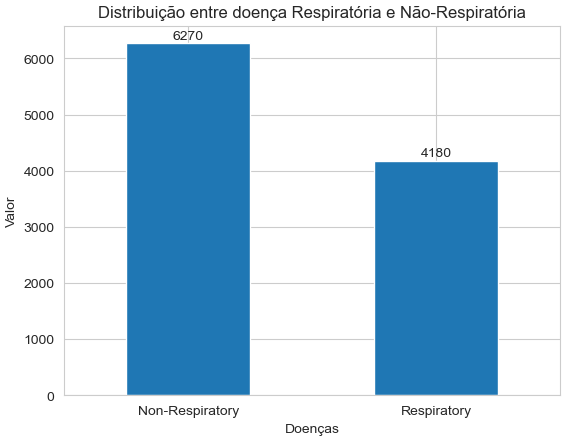
\includegraphics[width=0.6\linewidth]{grafico_doenca_respir}
	\caption{Distribuição de valores entre doença Respiratória e Não-Respiratória.}
	\label{fig:grafico_doenca_respir}
\end{figure}


\medskip

\subsubsection{\textbf{Exercício 4.3.2}}

Usando o método \textit{k-fold cross validation} desenvolvemos modelos de previsão de \textit{RespDisease} usando os seguintes métodos:

\medskip

\paragraph{Árvore de Decisão}

Começamos por definir os dados de entrada (X), que contêm os valores das colunas \textit{Affected Population}, \textit{Populated Area[km2]}, \textit{Air Pollution Average[ug/m3]} e \textit{Value}  e a variável objetivo (y) - \textit{RespDisease}.

De seguida, o \textit{dataset} é dividido na proporção 70-30 para treino e teste, com opção estratificada que garante que a proporção das classes se mantém balanceada entre treino e teste.

Passamos à aplicação do método de \textit{cross-validation}, escolhendo \textit{k = 10 folds}. Este irá armazenar a exatidão de cada \textit{fold} (\textit{k}).

Depois deste passo, treina-se o modelo final com todos os dados de treino e avalia-se no conjunto de teste separado inicialmente. Para isso, a função \textit{DecisionTreeClassifier - DTC} é utilizada, com critério de entropia. Na \figurename~\ref{fig:arvoreDecisaoCM} podemos visualizar a matriz de confusão resultante.

Para otimizar os parâmetros do modelo vamos tentar perceber qual o nível de profundidade que gera um melhor desempenho, iterando-a de 1 a 10, no algoritmo DTC e aplicando a validação cruzada.

Tomando o valor máximo da exatidão entre os diferentes níveis, verifica-se que o valor é máximo para o nível 10 de profundidade.

\begin{figure}[h]
	\centering
	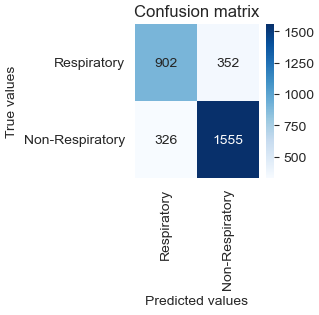
\includegraphics[width=0.5\linewidth]{arvoreDecisaoCM}
	\caption{Matriz de Confusão do modelo final.}
	\label{fig:arvoreDecisaoCM}
\end{figure}


\begin{table}[ht]
	\centering
	\caption{Exatidão da árvore de decisão por profundidade}
	\begin{tabular}{|c|c|}
		\hline
		\textbf{Profundidade da Árvore} & \textbf{Exatidão} \\
		\hline
		1  & 0.697 \\
		2  & 0.731 \\
		3  & 0.746 \\
		4  & 0.764 \\
		5  & 0.775 \\
		6  & 0.786 \\
		7  & 0.797 \\
		8  & 0.803 \\
		9  & 0.812 \\
		10 & 0.817 \\
		\hline
	\end{tabular}
	\label{tab:acc_tree_depth}
\end{table}

\medskip

\paragraph{Rede Neuronal}

Iniciamos a abordagem de forma análoga ao problema anterior, contudo, desta vez, fazemos a codificação da variável objetivo recorrendo ao \textit{LabelEncoder}, que lhe atribui valores binários (0 e 1).

Depois da separação dos dados em treino e teste, é feita a sua normalização recorrendo ao \textit{MinMaxScaler}, uma vez que as variáveis preditoras têm valores de magnitude muito distantes.

Definiram-se 2 configurações possíveis para a rede neuronal - uma com 50 neurónios na \textit{hidden layer} e a segunda com duas camadas - 100 e 50 na mesma \textit{layer}. Em comum, estas configurações têm a função ativação (\textit{tanh}), parâmetro \textit{alpha} (0,01), \textit{solver} (\textit{lbfgs}) e numero máximo de iterações ($max\_iter = 500$).

Outros parâmetros foram testados como o \textit{solver} "adam" mas obtiveram-se resultados inferiores de exatidão.

Entre estas duas configurações, a segunda (100,50) revelou-se um pouco melhor a nível de performance. 

\medskip

\paragraph{SVM}

O método de SVM, ao contrário da rede neuronal, necessita dos dados normalizados com o \textit{StandardScaler}. 

Para este algoritmo foi utilizado o método SVC - \textit{Support Vector Classification}, com parâmetros C = 10 e C = 100. e usando o \textit{Kernel rbf}.

Na \figurename~\ref{fig:arvoreDecisaoCM} podemos visualizar a comparação entre os dois modelos, em que C=100 obtém uma ligeira vantagem.

\begin{figure}[h]
	\centering
	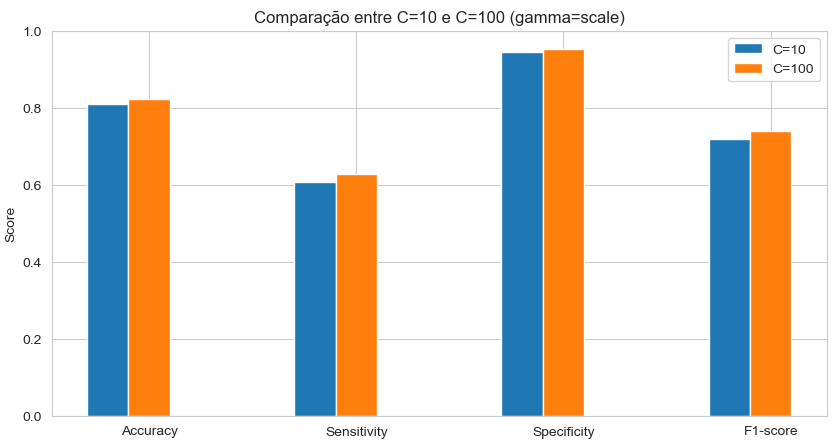
\includegraphics[width=0.7\linewidth]{svm_compare}
	\caption{Comparação entre resultados de SVM para C=10 e C=100.}
	\label{fig:svm_compare}
\end{figure}


\medskip

\paragraph{K-vizinhos-mais-próximos - kNN}

Neste algoritmo, a normalização dos dados é necessária, para isso, utilizámos o \textit{MinMaxScaler}, uma vez que estamos a falar de distância entre pontos para a kNN.

O \textit{KNeighborsClassifier} foi utilizado, testando entre 1 e 49, num passo de 2 (1,3,5...49). De todas as iterações, foi encontrada a que tem maior exatidão para k=5, visivel na \figurename~\ref{fig:kNN_exatidao_vs_k}.


\begin{figure}[h]
	\centering
	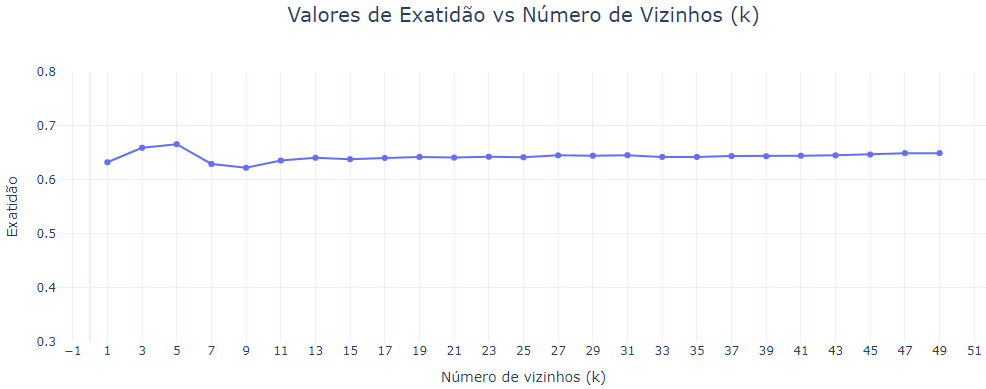
\includegraphics[width=0.9\linewidth]{kNN_exatidao_vs_k}
	\caption{kNN - Valores de exatidão em função de número de vizinhos \textit{k}.}
	\label{fig:kNN_exatidao_vs_k}
\end{figure}

\medskip

\subsubsection{\textbf{Exercício 4.3.3}}

Para cada modelo da questão anterior obtemos os seguintes valores médios e desvio padrão de Accuracy, Sensitivity, Specificity e F1:

\begin{table}[h]
	\centering
	\scriptsize
	\caption{Desempenho dos Modelos de Classificação}
	\begin{tabular}{|l|c|c|c|c|}
		\hline
		\textbf{Métrica} & \textbf{Decision Tree} & \textbf{NN (100,50)} & \textbf{SVM (C=100)} & \textbf{KNN} \\
		\hline
		Accuracy    & 0.784 ± 0.017   & 0.815 ± 0.013 & 0.823 ± 0.011 & 0.614 ± 0.029 \\
		Sensitivity & 0.775 ± 0.031   & 0.660 ± 0.031 & 0.629 ± 0.028 & 0.507 ± 0.026 \\
		Specificity & 0.775 ± 0.010   & 0.920 ± 0.010 & 0.952 ± 0.008 & 0.686 ± 0.059 \\
		F1 Score    & 0.775 ± 0.019   & 0.741 ± 0.019 & 0.739 ± 0.020 & 0.513 ± 0.017 \\
		\hline
	\end{tabular}
\end{table}


\medskip

\subsubsection{\textbf{Exercício 4.3.4}}

À luz dos resultados obtidos na questão anterior, percebemos que os modelos de SVM e NN têm a melhor \textit{accuracy} (exatidão), por isso, verificámos se existe uma diferença significativa no desempenho entre os dois, para um nível de significância de 5\% recorrendo ao teste \textit{t-stat}.

Como o\textit{ p-value} é inferior a 0,05, concluímos que há diferenças estatisticamente significativas entre os dois modelos.


\medskip

\subsubsection{\textbf{Exercício 4.3.5}}

A análise detalhada dos modelos revelou que o SVM com parâmetro \( C=100 \) apresenta o melhor desempenho global. Os principais pontos fortes incluem a maior \textit{accuracy} (82{,}3\%) entre todos os modelos, excelente \textit{specificity} (95{,}2\%) — o que indica menor número de falsos positivos — e baixa variabilidade, o que demonstra consistência nos resultados. Contudo, a principal limitação é a \textit{sensitivity} mais baixa (62{,}9\%), o que pode levar à perda de casos positivos.

A rede neural com arquitetura (100,50) foi a segunda melhor opção, alcançando uma \textit{accuracy} de 81{,}5\%, o melhor \textit{F1-score} (74{,}1\%), indicando bom equilíbrio entre precisão e sensibilidade, e uma \textit{specificity} elevada (91{,}9\%). No entanto, a \textit{sensitivity} foi inferior à da Árvore de Decisão.

A Árvore de Decisão destacou-se por apresentar a maior sensitivity (77{,}5\%), sendo a mais indicada em contextos onde é fundamental não deixar de identificar ocorrências relevantes. O modelo também apresentou equilíbrio geral entre as métricas, mas a \textit{accuracy} foi inferior à dos modelos SVM e NN.

Por fim, o modelo KNN demonstrou o pior desempenho geral, com a menor \textit{accuracy} (61{,}4\%), alta variabilidade entre os \textit{folds} e o \textit{F1-score} mais baixo (51{,}3\%), indicando um desempenho inferior em todos os aspetos avaliados.

\section*{Conclusões}

Este artigo analisou diferentes técnicas de aprendizagem automática aplicadas à previsão de mortes prematuras e à distinção de doenças respiratórias, utilizando dados de poluição atmosférica em países europeus. Foram implementados e comparados modelos de regressão (linear simples, linear múltipla, árvore de regressão, SVM e rede neural) e de classificação (árvore de decisão, rede neural, SVM e kNN), avaliando o desempenho de cada abordagem através de métricas estatísticas como MAE, RMSE, R\textsuperscript{2}, accuracy, sensitivity, specificity e F1-score.

A árvore de regressão apresentou o menor erro absoluto médio (MAE), demonstrando elevada precisão média nas previsões de mortes prematuras, enquanto a regressão linear múltipla mostrou maior robustez contra erros de maior magnitude, refletido pelo menor RMSE.

O modelo de rede neural destacou-se pelo maior coeficiente de determinação (R\textsuperscript{2}), evidenciando melhor capacidade de explicação da variância dos dados, especialmente em relações não lineares.

Nos modelos de classificação, o SVM com $C=100$ obteve a maior \textit{accuracy} (82,3\%) e especificidade (95,2\%), sendo o mais consistente e eficaz na identificação de doenças não respiratórias, embora com menor sensibilidade para os casos positivos.

A rede neural (100,50) foi a segunda melhor opção, com bom equilíbrio entre precisão e sensibilidade, enquanto a árvore de decisão destacou-se pela maior sensibilidade, sendo relevante em cenários onde é fundamental identificar corretamente todos os casos positivos.

O kNN apresentou o pior desempenho geral, com menor \textit{accuracy} e maior variabilidade entre os \textit{folds}, sugerindo menor adequação para este tipo de problema.

Em síntese, a escolha do modelo mais adequado depende do objetivo específico: maximizar precisão média, minimizar grandes erros ou equilibrar sensibilidade e especificidade. A análise reforça a importância da seleção criteriosa de algoritmos e da avaliação estatística rigorosa para problemas de previsão e classificação em contextos de saúde pública e poluição ambiental.


\begin{thebibliography}{00}
\bibitem{madureira2024aed}
Madureira, A., \& Matos, J. (2024). *Aulas T - Linear Regression and Tree Regression*. Instituto Superior de Engenharia do Porto (ISEP). Ano letivo 2024/2025.
\bibitem{madureira2024cv}
Madureira, A. (2024). *Aulas T - Cross Validation*. Instituto Superior de Engenharia do Porto (ISEP). Ano letivo 2024/2025.
\bibitem{moore2017}
Moore, D. S., McCabe, G. P., \& Craig, B. A. (2017). *Introduction to the Practice of Statistics* (9th ed.). New York: W. H. Freeman.
\bibitem{madureira2024}
Madureira, A., \& Matos, J. (2024). *Aulas T - Testes de Correlação*. Instituto Superior de Engenharia do Porto (ISEP). Ano letivo 2024/2025.
\bibitem{zar2005}
Zar, J. H. (2005). *Spearman Rank Correlation*. In Biostatistical Analysis (5th ed., pp. 383-387). Pearson Prentice Hall.
\bibitem{madureira2024adi}
Madureira, A. (2024). *Aulas T - Introduction to Machine Learning*. Instituto Superior de Engenharia do Porto (ISEP). Ano letivo 2024/2025.
\bibitem{madureira2024dt}
Madureira, A. (2024). *Aulas T - Decision Trees*. Instituto Superior de Engenharia do Porto (ISEP). Ano letivo 2024/2025.
\bibitem{ohekar_what_2023}
A.~Ohekar, ``What is the difference between a Decision Tree Classifier and a Decision Tree Regressor?,'' \emph{Medium}, Sep. 26, 2023. [Online]. Available: https://medium.com/@aaryanohekar277/what-is-the-difference-between-a-decision-tree-classifier-and-a-decision-tree-regressor-36641bd6559c [Accessed: Jun. 7, 2025].
\bibitem{refaeilzadeh_cross-validation_2009}
P.~Refaeilzadeh, L.~Tang, and H.~Liu, ``Cross-Validation,'' in \emph{Encyclopedia of Database Systems}, Springer, Boston, MA, 2009, pp. 532--538.
\bibitem{madureira2024nn}
Madureira, A. (2024). *Aulas T - Neural Networks*. Instituto Superior de Engenharia do Porto (ISEP). Ano letivo 2024/2025.
\bibitem{madureira2024svm}
Madureira, A. (2024). *Aulas T - Support Vector Machines*. Instituto Superior de Engenharia do Porto (ISEP). Ano letivo 2024/2025.
\bibitem{madureira2024knn}
Madureira, A. (2024). *Aulas T - kNN Algorithm*. Instituto Superior de Engenharia do Porto (ISEP). Ano letivo 2024/2025.
\bibitem{montgomery2021} 
Montgomery, D. C., Peck, E. A., \& Vining, G. G. (2021). 
\textit{Introduction to Linear Regression Analysis} (6ª ed.). Wiley.




\end{thebibliography}

\end{document}
